% Tested with pdfTeX in PDF mode.
\ifdefined\pdfoutput\pdfoutput=1\fi
\documentclass[11pt,a4paper]{article}
\usepackage[hmargin=28mm,vmargin=23mm]{geometry}
% Keep the first paragraph after a displayed section heading indented.
\usepackage{indentfirst}
\setlength{\parindent}{1.5em}
\usepackage{amsmath,amssymb,graphicx,booktabs}
\usepackage[hidelinks]{hyperref}
\usepackage{orcidlink}
\newcommand{\dd}{\mathrm{d}}
\newcommand{\sg}{\sigma}
\newcommand{\bc}{B_{\infty}}
\title{Five-point boundaries for a two-Higgs shift: from broken \(SU(2)\) to \(W^+W^-\to Zhh\)}
\author{Ming Li\,\orcidlink{0009-0007-7322-010X}\thanks{Corresponding author. E-mail: \href{mailto:by2419116@buaa.edu.cn}{\texttt{by2419116@buaa.edu.cn}}.}\\[0.4em]
  \normalsize School of Physics, Beihang University, Beijing 102206, China}
\date{}
\hypersetup{pdfauthor={Ming Li},pdftitle={Five-point boundaries for a two-Higgs shift in electroweak amplitudes}}
\begin{document}
\begingroup
\renewcommand{\textasteriskcentered}{\ensuremath{*}}
\maketitle
\endgroup

\begin{abstract}
In \(W^+W^-\to Zhh\), the two Higgs bosons can attach to the same
vector line or to different lines at the cubic gauge vertex. We compute
the tree-level boundary at complex infinity under a two-Higgs shift
that preserves the Higgs-pair momentum. The equal-mass broken \(SU(2)\)
theory exhibits a polarization cancellation of the different-arm
boundary. In the electroweak theory the charged
stationary currents are not conserved, and a term proportional to
\(m_Z^2-m_W^2\) lifts the different-arm cancellation when one charged
and the neutral polarization are orthogonal to the shift. The
cancellation for two shift-orthogonal charged polarizations survives.
Independent finite-\(R_\xi\) calculations check the full boundary
and unphysical-pole cancellation in both theories. A singlet scalar
can add a stationary resonance pole without changing the
different-arm polarization criterion.
\end{abstract}

\section{Introduction}
A complex deformation of external momenta reconstructs a tree amplitude
from its moving poles only if the contribution at infinity vanishes
\cite{BCF,BCFW}. Nonvanishing boundary contributions have been
computed for scalar and Yukawa theories \cite{FengBoundary}, and
boundary operators provide a systematic approach \cite{Jin}.
For massive gauge amplitudes, constructibility depends on the shift
and on the external spin states \cite{BallavManna,EmaMomentum}.
In particular, Franken and Schwinn \cite[Sec.~5.3.3]{Franken}
use three-line BCFW-type and Risager deformations involving vector
legs for mixed scalar--vector amplitudes in the transverse cases
covered there. Ema et al.\ \cite[Sec.~2]{Ema} use an all-line
deformation with fixed external wavefunctions, shifting vector
momenta along transverse directions. Their large-\(z\) power
counting gives constructibility at five and more points for the
renormalizable setting considered there. Neither statement requires
the boundary to vanish when only the Higgs momenta are shifted.

We hold all vector momenta and polarizations fixed and shift the two
Higgs momenta oppositely. This keeps \(m_{hh}^2\) fixed: the Higgs-pair
channel never generates a moving pole, and its stationary exchange
must be recovered through the boundary. The aim is therefore not to
find a more efficient constructible shift, but to separate this
physical pole from the different-arm contribution and determine
whether a polarization cancellation of the latter survives in
\(W^+W^-\to Zhh\). On-shell recursion for off-shell polarization
continuation is discussed in Ref.~\cite{Ke}; the known four-point
amplitude \cite{Aoude,Bachu,Balkin} and unitary-gauge tree currents
\cite{Dai} provide context but do not determine this different-arm
term. We first analyze equal-mass broken \(SU(2)\), then restore
hypercharge and allow scalar mixing. Section~\ref{sec:higher}
shows how the five-point boundary fixes a six-point stationary
residue without off-shell continuation. The external vectors are
physical and on shell; the topology split is in unitary gauge.

\section{Kinematics and the four-point tensor}
We take all momenta incoming, with metric \((+---)\). Denote the
three vector momenta and polarizations by \(k_i,e_i\), with
\(k_i^2=m^2\) and \(k_i\cdot e_i=0\), and the two Higgs momenta by
\(p,r\), with \(p^2=r^2=M^2\). Write \(H=p+r=-\sum_i k_i\).
The deformation is
\begin{equation}
 p(z)=p+zn,\qquad r(z)=r-zn,\qquad
 n^2=n\cdot p=n\cdot r=0.                                    \label{eq:shift}
\end{equation}
All contractions are bilinear also at complex momenta. We assume
generic kinematics with \(\ell_i=2k_i\cdot n\ne0\) and separated poles.
The boundary is the coefficient of \(z^0\) in the Laurent expansion
of \(A(z)\) at infinity. By Cauchy's theorem,
\begin{equation}
 A(0)=-\sum_{z_\alpha\ne0}\operatorname{Res}_{z=z_\alpha}
                 \frac{A(z)}{z}+B_\infty .
 \label{eq:cauchy}
\end{equation}
The sum is over the finite moving poles. The shift preserves \(H^2\),
so the boundary need not be local in all invariants.

Let \(a=g_2/2\), \(v=m/a\), \(g_h=2am\), and \(g_{hh}=2a^2\).
With the common cubic factor \(g_2 f^{abc}\) and overall phase
removed from the amplitudes with three vector legs, use
\begin{align}
 D(Q)&=Q^2-m^2, &
 U(Q)e&=\frac{e-Q(Q\cdot e)/m^2}{D(Q)},\\
 V(k;e)&=\sum_{(i,j,s)\,\mathrm{cyc}}
       (e_i\cdot e_j)(k_i-k_j)\cdot e_s .
\end{align}
We construct the amputated four-point current directly in unitary
gauge. The relevant terms in the gauge--Higgs Lagrangian
\cite{Denner} are
\[
 {\cal L}\supset \frac{m^2}{2}(1+h/v)^2 W_\mu^a W^{a\mu}
                  -\frac{M^2}{2v}h^3 .
\]
Take \(k\) on shell and let the other vector carry incoming momentum
\(-K=-(k+H)\), without imposing \(K^2=m^2\). Put \(p_z=p+zn\),
\(r_z=r-zn\), and \(L_x(z)=k+x_z\) for \(x=p,r\). With the adjoint
Kronecker delta and overall phase suppressed, the current is
\begin{equation}
 T_{\mu\nu}(z)=C_0g_{\mu\nu}
  +g_h^2\sum_{x=p,r}
  \frac{g_{\mu\nu}-L_{x\mu}(z)L_{x\nu}(z)/m^2}{D(L_x(z))}.
 \label{eq:amputated-current}
\end{equation}
The two terms in \(C_0\), given below, come from the \(WWhh\)
vertex and the \(h^*\to hh\) graph. No propagator of momentum \(K\)
is included in \(T_{\mu\nu}\). Imposing \(K^2=m^2\) and contracting
with physical polarizations instead gives the on-shell four-point
amplitude \cite{Balkin}; that amplitude is not used to choose the
off-shell current.

For the exchange with \(L=k+x\) and \(\sg_x=+1,-1\), take
vector arguments \(u,w\). Define
\(d=2k\cdot n\), \(N=u\cdot n\), \(P=w\cdot n\), \(X=u\cdot L\),
and \(Y=w\cdot L\). Polynomial division gives
\begin{equation}
 \frac{A_x(z)}{g_h^2}=
 -\frac{\sg_x NP}{m^2d}\,z
 +\frac{1}{m^2}\left[\frac{NP D(L)}{d^2}
                     -\frac{NY+PX}{d}\right]+O(z^{-1}) .
 \label{eq:division}
\end{equation}
The leading powers of the two exchanges cancel. The contact and
Higgs-pole terms are
\(C_0\,u\cdot w\), where
\begin{equation}
 C_0=g_{hh}+\frac{g_h(3M^2/v)}{H^2-M^2}.
 \label{eq:c0}
\end{equation}
Only the first term is local in \(H^2\).

\section{Five-point boundary and polarization condition}
There are 18 labelled trees in unitary gauge (Fig.~\ref{fig:topologies}).
\begin{figure}[tbp]
\centering
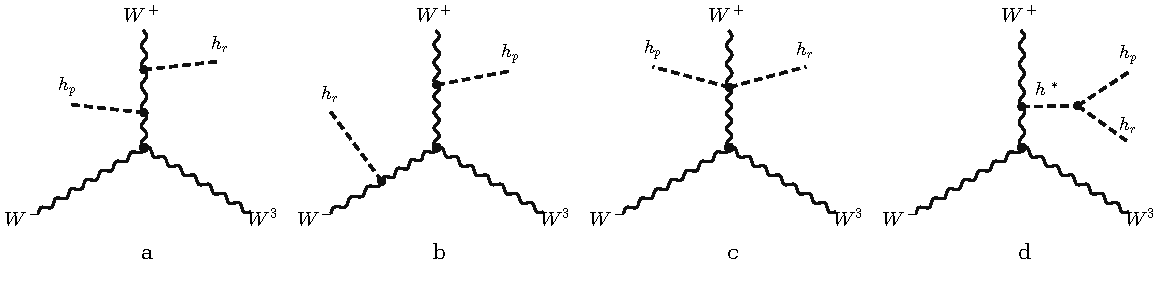
\includegraphics[width=\linewidth]{charged_topologies.pdf}
\caption{Representative five-point trees in unitary gauge:
(a) same-arm ordered emission, (b) cross-arm emission,
(c) quartic \(WWhh\) vertex, and (d) virtual Higgs splitting.
The corresponding numbers of labelled trees are \(6,6,3,3\).
The dashed lines labelled \(h_p,h_r\) carry \(p+zn,r-zn\),
respectively; the momentum of \(h^*\) is \(H=p+r\).}
\label{fig:topologies}
\end{figure}
For each gauge arm
there are two ordered emissions, one seagull and one virtual Higgs
splitting. The six remaining trees place the Higgs bosons on two
distinct arms. The four terms of Eq.~\eqref{eq:amputated-current},
attached to arm \(i\), account for precisely the four diagrams on
that arm. Their contribution at finite \(z\) is
\begin{equation}
 e_i^\mu T_{\mu\nu}(z)\,[U(K_i)J_i]^\nu,\qquad K_i=k_i+H ,
 \label{eq:current-sewing}
\end{equation}
where \(J_i\) is the cubic current of the other two physical vectors.
Contracting \(V\) gives \(K_i\cdot J_i=0\) for equal masses, so
\([U(K_i)J_i]^\nu=J_i^\nu/D(K_i)\) in this case. It does not put
\(K_i\) on shell.

Matching only to the on-shell amplitude would allow adding \(D(K_i)Y_{\mu\nu}\) to
\(T_{\mu\nu}\), with \(Y_{\mu\nu}\) regular at the root pole.
It would leave the on-shell four-point amplitude unchanged but
change Eq.~\eqref{eq:current-sewing} by
\(e_i^\mu Y_{\mu\nu}(g^{\nu\rho}-K_i^\nu K_i^\rho/m^2)J_{i\rho}\).
This term is regular at the root pole and does not vanish in
general, even when \(K_i\cdot J_i=0\). No such addition is made:
the fixed Lagrangian specifies the current, its quartic contact
is included once, and the six distinct-arm graphs are evaluated
separately. An off-shell rearrangement would have to retain any
compensating contact contributions in the full amplitude \cite{FearingScherer}.

For the constant term set
\begin{equation}
 R_i=\frac{n\cdot e_i}{\ell_i},\qquad
 F_i=\frac{H\cdot e_i-2R_i(M^2+k_i\cdot H)}{\ell_i},\qquad
 S_i=-\frac{R_i(2k_i+H)+nF_i}{m^2}.
\end{equation}
The same-arm and stationary boundary is a sum over arms of
\(V\) with momentum \(K_i\) and argument
\(U(K_i)(C_0e_i+g_h^2 S_i)\) on the indicated arm.

For a cross-arm assignment write
\(L_i=k_i+x+wn\), \(L_j=k_j+y-wn\) and \(b_i=L_i\cdot e_i\),
\(b_j=L_j\cdot e_j\), where \((x,y,w)=(p,r,z)\) or \((r,p,-z)\).
The contraction of the cubic vertex with \(L_i\) or \(L_j\) gives
\begin{align}
 V(L_i,L_j,k_s;L_i,e_j,e_s)
   &=-D(L_j)e_j\cdot e_s-b_jL_i\cdot e_s,\\
 V(L_i,L_j,k_s;e_i,L_j,e_s)
   &= D(L_i)e_i\cdot e_s-b_iL_i\cdot e_s,\\
 V(L_i,L_j,k_s;L_i,L_j,e_s)&=-m^2L_i\cdot e_s .
 \label{eq:ward}
\end{align}
Writing \(\rho_i=b_i/D(L_i)\), \(\rho_j=b_j/D(L_j)\), the
cross-arm term for one assignment is \(g_h^2\) times
\begin{equation}
 \frac{V(L_i,L_j,k_s;e_i,e_j,e_s)}{D(L_i)D(L_j)}
 +\frac{\rho_i e_j\cdot e_s-\rho_j e_i\cdot e_s
            +\rho_i\rho_j L_i\cdot e_s}{m^2}.
 \label{eq:cross-rational}
\end{equation}
The first term is \(O(z^{-1})\). On the \(i\)-th arm,
\(\rho_i=R_i+[(k_i+x)\cdot e_i-R_i D(k_i+x)]/(w\ell_i)+O(w^{-2})\);
the corresponding formula on the \(j\)-th arm uses \(-w\) and \(y\).
The \(O(w)\) terms from the last term in Eq.~\eqref{eq:cross-rational}
cancel upon exchanging the two Higgs attachments. The single-ratio
constants cancel in the cyclic sum. Combining the remaining constants
gives
\begin{equation}
 B_{\mathrm{cross}}=\frac{g_h^2}{m^2}
 \sum_{(i,j,s)\,\mathrm{cyc}}\!
 \left[R_iR_j(k_i-k_j)\cdot e_s+
        (n\cdot e_s)(R_jF_i-R_iF_j)\right].
 \label{eq:cross}
\end{equation}
This term requires no independent five-point interaction.

If \(n\cdot e_s=0\), the cyclic sum simplifies further:
\begin{equation}
 B_{\mathrm{cross}}=
 -\frac{2g_h^2 R_iR_j}{m^2\ell_s}
  e_s\cdot (\ell_j k_i-\ell_i k_j).
 \label{eq:onezero}
\end{equation}
Thus two shift-orthogonal polarizations are sufficient, but not
necessary. If exactly one is orthogonal, cancellation is equivalent
to the vanishing of the remaining contraction in Eq.~\eqref{eq:onezero}.
For generic momenta this selects a line in the two-dimensional
complex plane \(k_s^\perp\cap n^\perp\). This is not in general a
statement about a real linear polarization or a helicity eigenstate. As an exact check, set
\(m=g_2=1\) and choose
\[
\begin{aligned}
 k_1&=(3,2,2,0), & k_2&=(3,-2,2,0), &
 k_s&=(-\sqrt{17},0,-4,0),\\
 p&=H/2+(0,1/2,0,0), & r&=H-p, & n&=(0,0,1,i).
\end{aligned}
\]
Here \(M^2=p^2=r^2\) and \(s=3\).
For \(e_1=e_2=(0,0,0,1)\), choosing \(e_s=(0,1,0,0)\)
gives \(B_{\mathrm{cross}}=1/4\) in the stripped amplitude.
With the same momenta and \(e_1,e_2\), the complex physical
polarization \(e_s=(4,0,\sqrt{17},i\sqrt{17})\) gives zero;
neither \(n\cdot e_1\) nor \(n\cdot e_2\) vanishes.
The zero is unchanged by normalizing the polarization.

\paragraph{General polarizations.}
The condition \(n\cdot e_s=0\) is not required to classify the zeros.
Fix the momenta and the two physical polarizations \(e_i,e_j\), with
\((i,j,s)\) cyclic. Collecting the terms linear in \(e_s\) in
Eq.~\eqref{eq:cross} gives
\begin{align}
 \frac{m^2}{g_h^2}B_{\rm cross}&=e_s\cdot Q_s,\qquad
 Q_s=R_iR_j(k_i-k_j)+\beta_s H+\gamma_s n,\nonumber\\
 \beta_s&=\frac{(\ell_j-\ell_i)R_iR_j}{\ell_s},\nonumber\\
 \gamma_s&=R_jF_i-R_iF_j
  +\frac{R_j(k_j-k_s)\cdot e_i+R_i(k_s-k_i)\cdot e_j}{\ell_s}
  \nonumber\\
 &\quad+\frac{\ell_iR_iF_j-\ell_jR_jF_i
           -2(M^2+k_s\cdot H)\beta_s}{\ell_s}.
 \label{eq:general-cross-covector}
\end{align}
Only \(Q_s^\perp=Q_s-k_s(k_s\cdot Q_s)/m^2\) enters this
contraction. If \(Q_s^\perp=0\), every physical \(e_s\) gives
a zero. Otherwise the zeros form a two-dimensional complex
subspace of the three-dimensional physical polarization space
\(k_s^\perp\), or a projective line when the overall polarization
scale is removed. Varying the first two polarizations gives all
triples with \(B_{\rm cross}=0\). For real kinematics and real linear
polarizations the corresponding space has dimension \(3-r\), where
\(r\) is the real rank of the two linear forms obtained from
\(\operatorname{Re}Q_s^\perp\) and \(\operatorname{Im}Q_s^\perp\)
on \(k_s^\perp\). Thus the real dimension is one, two or three, not
necessarily the real counterpart of the complex dimension above.
For a fixed helicity basis, each basis state must be tested
separately.

This characterization recovers Eq.~\eqref{eq:onezero} upon imposing
\(n\cdot e_s=0\). It also gives zeros with all three
\(n\cdot e_a\ne0\): in the same equal-mass kinematics and with the same
\(e_1,e_2\) as above, choose the real \(e_s=(4,0,\sqrt{17},0)\).
Then \(Q_s\) is proportional to \(k_1-k_2\), and the different-arm
boundary vanishes.

The condition on the cross contribution does not remove the
stationary Higgs pole. In the full boundary,
\begin{equation}
 \mathop{\rm Res}_{H^2=M^2}\bc
    =\frac{3M^2}{v} A_4(W^+W^-W^3h).
 \label{eq:fixed-higgs-residue}
\end{equation}
The right-hand side does not vanish identically. For example, at
right-angle two-body kinematics with the initial vector momenta
along the \(z\) axis, choose the two initial polarizations along
\(y\) and the final vector polarization along \(z\). The reduced
four-point amplitude is \(2g_h|\boldsymbol{k}_1|
\sum_i D(K_i)^{-1}\). At large initial-vector energy \(E\),
the sum is \(-3/(4E^2)+O(E^{-4})\), so the residue is not identically
zero. The pole
statement is analytic; it does not require a real \(h\to hh\) decay.
For fixed regular kinematics the moving poles alone reconstruct
the amplitude precisely when \(B_{\rm same}+B_{\rm cross}=0\).
As a check of the sign in Eq.~\eqref{eq:cauchy}, we computed the six
moving residues for each of 20 phase-space points and both null
directions, using the three physical intermediate spin states.
Across these 40 deformations the largest scaled reconstruction
difference with the boundary included was \(7.84\times10^{-15}\).

\section{Cancellation of the gauge poles}
\label{sec:gauge}
Use a Cartesian Higgs doublet
\(\Phi=(v+h+i\chi^a\sigma^a)(0,1)^T/\sqrt 2\) and
\(D_\mu=\partial_\mu-iaW_\mu^a\sigma^a\).
The gauge-fixing function is
\(F^a=\partial\cdot W^a+\xi m\chi^a\).
The derivative interactions needed in addition to the unitary-gauge
vertices are
\begin{equation}
 aW_\mu^a(\chi^a\partial^\mu h-h\partial^\mu\chi^a)
 +a\epsilon^{abc}W_\mu^a\chi^b\partial^\mu\chi^c.
 \label{eq:gold}
\end{equation}
There is no \(WW\chi\) vertex. With no external ghosts, ghost-number
flow would require a closed ghost line, so ghosts do not occur
in this tree amplitude.

Let \(E(Q)=Q^2-\xi m^2\). With the factor \(-i\) removed from
the vector propagator, its finite-gauge form is
\begin{equation}
 U_\xi(Q)=U(Q)+\frac{QQ}{m^2 E(Q)}.
\end{equation}
On a stationary root \(K_i\) the difference vanishes after
contraction with \(J_i\). For an ordered same-arm emission it
adds a longitudinal term proportional to
\[
 \frac{g_h^2(L\cdot e_i)(L\cdot J_i)}{m^2 E(L)D(K_i)} .
\]
The derivative \(Wh\chi\) vertices in Eq.~\eqref{eq:gold} give
the negative of this term, since \(g_h/m=2a\).
This accounts for the six single-Goldstone trees.

For a cross-arm assignment, use
Eqs.~\eqref{eq:ward} to expand the difference between
\(U_\xi(L_i)U_\xi(L_j)\) and \(U(L_i)U(L_j)\).
Suppressing the overall \(g_h^2/m^2\), the difference is
\begin{equation}
 -\frac{b_i}{E(L_i)} e_j\cdot e_s
 +\frac{b_j}{E(L_j)} e_i\cdot e_s
 -\frac{b_i b_j}{E(L_i)E(L_j)}L_i\cdot e_s .
 \label{eq:difference}
\end{equation}
The last term cancels the tree with two Goldstone lines joining a
\(W\chi\chi\) vertex. The first two terms cancel after summing attachments:
for each fixed Higgs and arm, its two possible partners give the same
factor with opposite sign. The proof holds at finite complex \(z\),
so the full shifted amplitudes agree as rational functions. Their
boundary coefficients and physical poles agree, and the poles at
\(L_i^2=\xi m^2\) are removable. The statement concerns the full
amplitude; the separate diagrams are gauge dependent.
The usual vector--Goldstone relation is discussed in
Ref.~\cite{Chen}; the explicit cancellation above also exhibits the
role of the cyclic sum.

We checked this result by independently enumerating labelled trees
from the Cartesian action and evaluating the standard finite-
\(\xi\) propagator without making a unitary subtraction. The recursion
generates 18 trees with no Goldstone line, six with one, and six
with two. For six real phase-space points, both null shifts and
\(\xi=0.31,1.7,4.2\), we compared the signed amplitude at finite
\(z\), the coefficient at infinity, and the six physical and six
candidate unphysical residues. The tests include external longitudinal
polarization and retain the separately nonzero Goldstone and vector
pieces in the archived data. The largest scaled discrepancies are
\(2.36\times 10^{-14}\) for the finite-shift amplitude,
\(3.22\times 10^{-15}\) for the boundary and
\(4.26\times 10^{-10}\) for the physical residues. The largest
scaled residue at an unphysical pole is \(4.64\times 10^{-10}\).
The scale in each comparison is the largest of unity, the
absolute reference and the sum of absolute values of the separately
computed contributions. The small residuals reflect floating-point
contour evaluation rather than a nonzero analytic residue.
Independently, exact scalar-product reductions in FeynCalc
10.2.1 (development version) \cite{FeynCalc,FeynCalc102} reproduce the cubic
contractions and the cancellations above. Removing the
two-Goldstone graph leaves a nonzero numerator over the
unphysical denominators; this provides a sign and omission check.
This symbolic reduction uses the derived vertices and does not
generate the diagrams.

\section{Electroweak \texorpdfstring{\(W^+W^-\to Zhh\)}{W+W- to Zhh}}
We now restore hypercharge and keep the same deformation. In this
section \(k_i^2=m_i^2\), with the cyclic order \(+,-,Z\). We remove
the common \(WWZ\) coupling and overall phase. The \(hV_iV_i\) and
\(hhV_iV_i\) vertex strengths in the mass basis are \(g_i=2m_i^2/v\)
and \(d_i=2m_i^2/v^2\), respectively, with the charged fields paired
at each vertex \cite{Denner}. In unitary gauge the 18 trees still fall
into the same four classes. A photon does not replace an internal
neutral vector in these trees because there is no tree-level
\(hZ\gamma\) or \(hhZ\gamma\) vertex.

\paragraph{Same arm.}
Let \(D_i(Q)=Q^2-m_i^2\) and
\(U_i(Q)e=[e-Q(Q\cdot e)/m_i^2]/D_i(Q)\).
The four-point insertion follows directly from the \(hV_iV_i\)
and \(hhV_iV_i\) vertices, with both vector indices open before
contraction. In particular, the contact term is included once and
no on-shell condition is imposed on the stationary internal vector.
Polynomial division of its two ordered exchanges yields the boundary
\begin{equation}
 X_i=\left(d_i+\frac{3M^2 g_i}{v(H^2-M^2)}\right)e_i
      -\frac{g_i^2}{m_i^2}\bigl[R_i(2k_i+H)+nF_i\bigr] .
 \label{eq:ew-x}
\end{equation}
The corresponding contribution is obtained by inserting
\(U_i(K_i)X_i\) into \(V\) with momentum \(K_i=k_i+H\).
For the cubic current \(J_i\), defined by \(V=J_i\cdot e_i\) at the
stationary vertex, the three-vector current identity
\cite[Eq.~(19)]{Ke} gives
\begin{equation}
 K_i\cdot J_i=(m_s^2-m_j^2)e_j\cdot e_s.
 \label{eq:ew-root}
\end{equation}
Thus only the neutral root is conserved for general polarizations.
Replacing \(U_i(K_i)\) by its metric term on a charged root would
miss \(- (K_i\cdot X_i)(K_i\cdot J_i)/(m_i^2 D_i(K_i))\).

\paragraph{Different arms.}
Define
\begin{equation}
 {\cal C}_{ijs}=R_iR_j(k_i-k_j)\cdot e_s
            +(n\cdot e_s)(R_jF_i-R_iF_j).
 \label{eq:ew-C}
\end{equation}
Expanding both Higgs assignments and then summing over the
three pairs of arms gives (see Appendix~\ref{app:ew-cross})
\begin{align}
 B_{\rm cross}^{\rm EW}
  ={}&\frac{4}{v^2}\sum_{\rm cyc}(m_i^2+m_j^2-m_s^2){\cal C}_{ijs}
      \nonumber\\
     &+\frac{8}{v^2}\sum_{\rm cyc}(m_j^2-m_s^2)R_i(e_j\cdot e_s).
 \label{eq:ew-cross}
\end{align}
For equal masses Eq.~\eqref{eq:ew-cross} reduces to
Eq.~\eqref{eq:cross}. If both charged polarizations are orthogonal to
\(n\), it vanishes even at \(m_Z\ne m_W\). If instead
\(n\cdot e_-=n\cdot e_Z=0\), the first line vanishes but the second
gives
\begin{equation}
 B_{\rm cross}^{\rm EW}
   =-\frac{8(m_Z^2-m_W^2)}{v^2}\,R_+(e_-\cdot e_Z).
 \label{eq:ew-obstruction}
\end{equation}
The example with \(W^+\) and \(Z\) orthogonal follows by interchanging
the charged legs, with the sign fixed by the cyclic vertex convention.
The new term in Eq.~\eqref{eq:ew-obstruction} is proportional to \(g'^2\), since
\(m_Z^2-m_W^2=g'^2v^2/4\) at tree level.

For general polarizations, fix \(e_i,e_j\) and let \((i,j,s)\)
be cyclic. Define \(\omega_s=m_i^2+m_j^2-m_s^2\) and
\(\Delta_s=m_i^2-m_j^2\), with \(\omega_i,\omega_j,\Delta_i,\Delta_j\)
given by cyclic rotation. The explicit linear form is
\begin{align}
 \frac{v^2}{4}B_{\rm cross}^{\rm EW}
   &=e_s\cdot Q_s^{\rm EW},\nonumber\\
 Q_s^{\rm EW}
   &=\omega_s R_iR_j(k_i-k_j)+\beta_s^{\rm EW}H
      +\gamma_s^{\rm EW}n
      +2\Delta_i R_i e_j+2\Delta_j R_j e_i,\nonumber\\
 \beta_s^{\rm EW}
   &=\frac{(\omega_j\ell_j-\omega_i\ell_i)R_iR_j}{\ell_s},\nonumber\\
 \gamma_s^{\rm EW}
   &=\omega_s(R_jF_i-R_iF_j)
    +\frac{\omega_i R_j(k_j-k_s)\cdot e_i
          +\omega_j R_i(k_s-k_i)\cdot e_j}{\ell_s}\nonumber\\
   &\quad+\frac{\omega_i\ell_i R_iF_j-\omega_j\ell_j R_jF_i
       -2(M^2+k_s\cdot H)\beta_s^{\rm EW}
       +2\Delta_s(e_i\cdot e_j)}{\ell_s}.
 \label{eq:ew-covector}
\end{align}
The criterion is \(e_s\cdot Q_s^{{\rm EW},\perp}=0\), where
\(Q_s^{{\rm EW},\perp}=Q_s^{\rm EW}-k_s(k_s\cdot Q_s^{\rm EW})/m_s^2\).
The complex and real kernels have the same dimension rules as
in Sec.~3. For equal masses \(Q_s^{\rm EW}=m^2 Q_s\).

As an exact check, choose \(m_W=1\), \(v=2\),
\(k_+=(3,2,2,0)\), \(k_-=(3,-2,2,0)\), and
\(k_Z=(-25/6,0,-4,0)\). Set \(p=H/2+(0,1/4,0,0)\), \(r=H-p\)
and \(n=(0,0,1,i)\), with
\(e_+=(0,0,0,1)\), \(e_-=(-2/3,1,0,0)\) and \(e_Z=(0,1,0,0)\).
Here \(m_Z^2=49/36\), both \(e_-\) and \(e_Z\) are orthogonal to
\(n\), and a direct Laurent expansion of the six different-arm
graphs gives \(13i/72\), as in Eq.~\eqref{eq:ew-obstruction}.
The direct sum of the other twelve gives \(-13109i/13200\).
The separation is a statement about diagram classes in unitary
gauge under this shift, not a zero of a physical cross section.
At the stationary Higgs pole, the electroweak residue similarly
factorizes into the trilinear Higgs coupling and the on-shell
\(W^+W^-\to Zh\) amplitude \cite[Sec.~4.3]{Bachu}.

\paragraph{Finite-gauge check.}
For physical on-shell external states, the full tree amplitude in
two gauges agrees on an open set of real kinematics. The amplitudes
are rational functions of the momenta and polarizations, so this
identity continues to the complex on-shell kinematics of the
Higgs shift. Taking the Laurent coefficient then gives the same
\(B_\infty\) in both gauges. This argument applies to the sum of
all diagrams; the mass-splitting term in
Eq.~\eqref{eq:ew-obstruction} refers to the unitary-gauge split.

We independently constructed the electroweak tree amplitude in
linear \(R_\xi\) gauge with separate parameters \(\xi_W,\xi_Z\).
In a Cartesian Higgs basis, the neutral doublet generator is
\(T_Z=(g c_W\sigma^3-g's_W\mathbf{1})/2\).
The anticommutators of the doublet generators in
\((D_\mu\Phi)^\dagger D^\mu\Phi\) give both \(ZW^\pm G^\mp\)
and \(ZW^\pm G^\mp h\) vertices in addition to the equal-mass
interactions. In particular, the \(ZW^\pm G^\mp\) strength is
proportional to \((m_Z^2-m_W^2)/m_W\) after removing the common
\(WWZ\) coupling. Omitting such terms would not implement the
finite-gauge check for the split-mass theory.

A labelled recursion with the Cartesian vertices gives 52 trees
in the \(W^1W^2Zhh\) projection: 18 without a Goldstone propagator,
24 with one, and 10 with two. We compare its sum with the
unitary-gauge result for \(m_W=80.377\), \(m_Z=91.1876\),
\(M=125.25\) and \(v=246.22\), in GeV, taking \(c_W=m_W/m_Z\).
Six kinematic points, including longitudinal polarizations,
were tested with both null shifts and
\((\xi_W,\xi_Z)=(0.31,1.7),(1.9,0.43),(3.2,4.2)\).
The largest scaled differences are \(8.41\times10^{-14}\) for
144 finite-shift amplitudes, \(2.13\times10^{-14}\) for
36 boundaries and \(3.40\times10^{-14}\) for 216 physical
moving residues. All 216 candidate unphysical moving residues
are consistent with zero, with a maximum scaled magnitude
\(1.02\times10^{-14}\). Laurent checks at the stationary
root denominators, treating the gauge parameter as the
complex variable, give a maximum scaled residue
\(4.83\times10^{-12}\). As in Sec.~\ref{sec:gauge},
the comparison is of the complete amplitude, not of
individual topology classes. Deleting the charged
Goldstone graphs spoils the agreement.

\section{Singlet scalar mixing}
In a real singlet extension, write the doublet fluctuation as
\(h_D=c_\theta h_1+s_\theta h_2\), where \(h_1\) is the light Higgs.
The kinetic term rescales each \(h_1VV\) vertex by \(c_\theta\)
and each \(h_1h_1VV\) vertex by \(c_\theta^2\).
There is no \(Zh_1h_2\) vertex in this extension. Hence the ordered,
contact and different-arm terms for \(W^+W^-Zh_1h_1\) are their SM
counterparts times \(c_\theta^2\). Defining
\(\lambda_{a11}=\partial_{h_a}\partial_{h_1}^2{\cal V}|_{\rm vac}\)
for the scalar potential \({\cal V}\), the stationary coefficient
on arm \(i\) is instead
\begin{equation}
 c_\theta^2d_i+
 g_i\left[
 \frac{c_\theta\lambda_{111}}{H^2-m_1^2}+
 \frac{s_\theta\lambda_{211}}{H^2-m_2^2}
 \right].
 \label{eq:singlets}
\end{equation}
The heavy exchange is a fixed pole because the shift keeps \(H^2\)
unchanged. Its residue is \(\lambda_{211}\) times the on-shell
amplitude for \(W^+W^-\to Zh_2\), in the same phase convention.
In the alignment limit \(c_\theta=1\), \(s_\theta=0\) and
\(\lambda_{111}=3m_1^2/v\), Eq.~\eqref{eq:singlets}
returns the SM. The resonant production mechanism is known
\cite{Kotwal}; the point here is that the resonance belongs entirely
to the boundary, without changing the different-arm polarization
criterion.

\section{From five points to higher-point boundaries}
\label{sec:higher}
Two features of the construction extend beyond five points.
First, on any tree an internal edge carries the shift if and only
if cutting it separates the two marked Higgs legs. These edges form
the unique path between the Higgs insertions. All subtrees attached to
that path carry momenta independent of \(z\), and can be evaluated once
as ordinary tree currents. This is the tree-level separation
underlying the hard-line expansion of Ref.~\cite{ArkaniKaplan}. The different-arm topology at five points
is the instance in which two shifted vector lines meet at a cubic
gauge vertex. At higher points such a vertex can have an entire
unshifted current attached to it. The path may also pass through
quartic vertices or several successive gauge vertices. The separation
into a shifted path and fixed currents therefore persists, but the
five-point polarization criterion is not a higher-point identity.
In computing the constant term one must retain subleading terms on
the path whenever they multiply positive powers of \(z\).

Second, the lower-point boundary fixes residues of the higher-point
boundary on stationary physical poles. Let \(P\) be the momentum
of such a channel, and let the left subamplitude contain both
shifted legs. At generic kinematics, with other poles separated and
the leading shifted denominators nonzero on this locus, tree
factorization gives
\begin{equation}
 \mathop{\rm Res}_{P^2=m_I^2} B_N
 =\sum_{\lambda_I} B_L(P,\lambda_I)\, A_R(-P,\lambda_I).
 \label{eq:fixed-factorization}
\end{equation}
The product is understood in a dual basis of intermediate physical
states. To obtain this equation, factorize \(A_N(z)\) at the fixed
pole and take its \(z^0\) coefficient. The right subamplitude and the
intermediate spin sum are independent of \(z\), so only the shifted
left subamplitude contributes a boundary operation. The Higgs pole
in Eq.~\eqref{eq:fixed-higgs-residue} is the case \(B_L=A_3(hhh)\).

For example, in the all-incoming \(W^+W^-Z_1Z_2hh\) amplitude
consider the channel \(P=k_{W^+}+k_{Z_1}\). At the stationary
pole \(P^2=m_W^2\), the unshifted factor is
\(A_3(W^+,Z_1,W^-(-P))\); the shifted factor is the five-point
boundary for \(W^+(P)W^-Z_2hh\) computed above. With the cubic
couplings restored, Eq.~\eqref{eq:fixed-factorization} gives this
six-point residue without an off-shell continuation of the
five-point result. It does not determine the full six-point
boundary: terms regular on the stationary poles, including
contributions from new shifted paths, are not fixed by their
residues. At fixed multiplicity one can use the residue equations
as constraints and compute the remaining terms from the shifted
tree currents. This supplements, rather than replaces, other
constructible shifts or general boundary-operator methods
\cite{Ema,Jin}.

\section{Conclusions}
For the fixed-pair-momentum shift, the different-arm boundary is not
captured by inserting a four-point tensor on a single gauge arm. The
equal-mass result gives a polarization cancellation that is only
partly inherited by \(W^+W^-\to Zhh\): the zero for both charged
polarizations orthogonal to the shift survives, but the mixed
charged--neutral case acquires a mass-splitting term. Singlet mixing,
by contrast, rescales the different-arm term and can add a fixed
scalar pole. These results distinguish vector-mass and scalar-pole
effects for the specified shift. They do not constrain constructibility
under an all-line transverse deformation or imply a cross-section zero.

\appendix
\section{Expansion of the electroweak different-arm graphs}
\label{app:ew-cross}
For a cyclic triple \((i,j,s)\), let
\(L_i=k_i+x+wn\) and \(L_j=k_j+y-wn\).
The two assignments are \((x,y,w)=(p,r,z)\) and \((r,p,-z)\).
Write \(D_i=D_i(L_i)\), \(D_j=D_j(L_j)\) and
\(\rho_a=L_a\cdot e_a/D_a\). With the common \(WWZ\)
factor still removed, the amplitude of one graph is
\begin{align}
 \frac{{\cal A}_{ijs}(x,y;w)}{g_i g_j}
 &=\frac{V(L_i,L_j,k_s;e_i,e_j,e_s)}{D_iD_j}
   +\frac{\rho_i}{m_i^2}\left(1+\frac{m_j^2-m_s^2}{D_j}\right)
          e_j\cdot e_s\nonumber\\
 &\quad-\frac{\rho_j}{m_j^2}\left(1+\frac{m_i^2-m_s^2}{D_i}\right)
          e_i\cdot e_s
   +\frac{\omega_s}{m_i^2m_j^2}\rho_i\rho_j L_i\cdot e_s.
 \label{eq:ew-assignment-exact}
\end{align}
Indeed the longitudinal part on arm \(i\) contracts the cubic
vertex to \((m_s^2-L_j^2)e_j\cdot e_s
-(L_j\cdot e_j)(L_i\cdot e_s)\); on arm \(j\), the result is
\((L_i^2-m_s^2)e_i\cdot e_s
-(L_i\cdot e_i)(L_i\cdot e_s)\). The double contraction gives
\(-m_s^2 L_i\cdot e_s\). These are Eq.~\eqref{eq:ward}
with the mass of the unshifted leg kept explicit. The first term of
Eq.~\eqref{eq:ew-assignment-exact} and the explicit mass differences
divided by \(D_i\) or \(D_j\) contribute only at \(O(z^{-1})\).

For an unshifted Higgs momentum \(x\), define
\[
 c_a(x)=\frac{(k_a+x)\cdot e_a-R_aD_a(k_a+x)}{\ell_a},
 \qquad c_a(p)+c_a(r)=F_a .
\]
Then \(\rho_i=R_i+c_i(x)/w+O(w^{-2})\) and
\(\rho_j=R_j-c_j(y)/w+O(w^{-2})\).
Using \(g_i=2m_i^2/v\), the two full expansions through the
constant term are
\begin{align}
 \frac{v^2}{4}{\cal A}_{ijs}(p,r;z)
 &=S_{ijs}+\omega_s\Big[
     zR_iR_j(n\cdot e_s)+R_iR_j(k_i+p)\cdot e_s
       \nonumber\\
 &\hspace{25mm}+(n\cdot e_s)\big(R_jc_i(p)-R_ic_j(r)\big)\Big]
       +O(z^{-1}),\nonumber\\
 \frac{v^2}{4}{\cal A}_{ijs}(r,p;-z)
 &=S_{ijs}+\omega_s\Big[
     -zR_iR_j(n\cdot e_s)+R_iR_j(k_i+r)\cdot e_s
       \nonumber\\
 &\hspace{25mm}+(n\cdot e_s)\big(R_jc_i(r)-R_ic_j(p)\big)\Big]
       +O(z^{-1}),
 \label{eq:ew-assignment-expand}\\
 S_{ijs}&=m_j^2 R_i(e_j\cdot e_s)-m_i^2 R_j(e_i\cdot e_s).
 \nonumber
\end{align}
The \(O(z)\) terms cancel within each pair. In the sum of the
constants, \((2k_i+H)\cdot e_s=(k_i-k_j)\cdot e_s\), so the
weighted pair gives \(\omega_s{\cal C}_{ijs}\). The remaining
single-ratio terms give \(2S_{ijs}\) per pair, and the cyclic sum
satisfies
\[
 \sum_{\rm cyc} S_{ijs}
   =\sum_{\rm cyc}(m_j^2-m_s^2)R_i(e_j\cdot e_s).
\]
This yields Eq.~\eqref{eq:ew-cross}. When \(m_i=m_j=m_s=m\),
the last sum vanishes identically and \(\omega_s=m^2\), so
\(4m^2/v^2=g_h^2/m^2\) and Eq.~\eqref{eq:cross} follows.

\section*{Data availability}
No external datasets were used in this study.

% Before submission, insert author-confirmed funding and competing-interest
% declarations as applicable, and the required generative-AI disclosure
% before the references. See Author_Preflight.md in the source bundle.
\begingroup\small
\begin{thebibliography}{99}
\setlength{\itemsep}{0pt}
\setlength{\parsep}{0pt}
\bibitem{BCF} R. Britto, F. Cachazo and B. Feng,
Nucl. Phys. B \textbf{715} (2005) 499--522,
\href{https://arxiv.org/abs/hep-th/0412308}{arXiv:hep-th/0412308}.
\bibitem{BCFW} R. Britto, F. Cachazo, B. Feng and E. Witten,
Phys. Rev. Lett. \textbf{94} (2005) 181602,
\href{https://arxiv.org/abs/hep-th/0501052}{arXiv:hep-th/0501052}.
\bibitem{FengBoundary} B. Feng, J. Wang, Y. Wang and Z. Zhang,
JHEP \textbf{01} (2010) 019,
\href{https://arxiv.org/abs/0911.0301}{arXiv:0911.0301}.
\bibitem{Jin} Q. Jin and B. Feng, JHEP \textbf{04} (2016) 123,
\href{https://arxiv.org/abs/1507.00463}{arXiv:1507.00463}.
\bibitem{BallavManna} S. Ballav and A. Manna, Nucl. Phys. B
\textbf{983} (2022) 115935,
\href{https://arxiv.org/abs/2109.06546}{arXiv:2109.06546}.
\bibitem{Franken} R. Franken and C. Schwinn,
JHEP \textbf{02} (2020) 073,
\href{https://arxiv.org/abs/1910.13407}{arXiv:1910.13407}.
\bibitem{EmaMomentum} Y. Ema, T. Gao, W. Ke, Z. Liu, K.-F. Lyu and I. Mahbub,
Phys. Rev. D \textbf{110} (2024) 105003,
\href{https://arxiv.org/abs/2403.15538}{arXiv:2403.15538}.
\bibitem{Ema} Y. Ema, T. Gao, W. Ke, Z. Liu, K.-F. Lyu and I. Mahbub,
Phys. Rev. D \textbf{110} (2024) 105002,
\href{https://arxiv.org/abs/2407.14587}{arXiv:2407.14587}.
\bibitem{Ke} W. Ke, Z. Liu and I. Mahbub,
\href{https://arxiv.org/abs/2611.13096}{arXiv:2611.13096}.
\bibitem{Dai} L. Dai, K. Melnikov and F. Caola,
JHEP \textbf{04} (2012) 095,
\href{https://arxiv.org/abs/1201.1523}{arXiv:1201.1523}.
\bibitem{Aoude} R. Aoude and C. S. Machado,
JHEP \textbf{12} (2019) 058,
\href{https://arxiv.org/abs/1905.11433}{arXiv:1905.11433}.
\bibitem{Balkin} R. Balkin, G. Durieux, T. Kitahara, Y. Shadmi and
Y. Weiss, JHEP \textbf{03} (2022) 129,
\href{https://arxiv.org/abs/2112.09688}{arXiv:2112.09688}.
\bibitem{Chen} J. Chen, K. Hagiwara, J. Kanzaki and K. Mawatari,
Eur. Phys. J. C \textbf{83} (2023) 922,
\href{https://doi.org/10.1140/epjc/s10052-023-12093-7}{doi:10.1140/epjc/s10052-023-12093-7}.
\bibitem{FeynCalc}
V. Shtabovenko, R. Mertig and F. Orellana,
Comput. Phys. Commun. \textbf{306} (2025) 109357,
\href{https://doi.org/10.1016/j.cpc.2024.109357}{doi:10.1016/j.cpc.2024.109357}.
\bibitem{FeynCalc102} V. Shtabovenko,
\href{https://arxiv.org/abs/2512.19858}{arXiv:2512.19858}.
\bibitem{Denner} A. Denner, Fortschr. Phys. \textbf{41} (1993) 307--420,
\href{https://arxiv.org/abs/0709.1075}{arXiv:0709.1075}.
\bibitem{Kotwal} A. V. Kotwal, M. J. Ramsey-Musolf, J. M. No and P. Winslow,
Phys. Rev. D \textbf{94} (2016) 035022,
\href{https://arxiv.org/abs/1605.06123}{arXiv:1605.06123}.
\bibitem{Bachu} B. Bachu and A. Yelleshpur, JHEP \textbf{08} (2020) 039,
\href{https://arxiv.org/abs/1912.04334}{arXiv:1912.04334}.
\bibitem{FearingScherer} H. W. Fearing and S. Scherer,
Phys. Rev. C \textbf{62} (2000) 034003,
\href{https://arxiv.org/abs/nucl-th/9909076}{arXiv:nucl-th/9909076}.
\bibitem{ArkaniKaplan} N. Arkani-Hamed and J. Kaplan, JHEP \textbf{04} (2008) 076,
\href{https://arxiv.org/abs/0801.2385}{arXiv:0801.2385}.
\end{thebibliography}
\endgroup
\end{document}
